\chapter{Implementing SMART}

As has been said, the SMART implementation is one of the main purposes of this thesis. In this chapter, more details of the SMART project will be presented and all information about how it was implemented. 

A Github repository\footnote{\url{https://github.com/capellaresumo/MAC0499}} all the source code used during the implementation. Additionally, there is instruction for how to build and test the project. 

\section{Premises}

In the main article a few assertions are made to informal proof the SMART security. These assertions were used to drive the construction of the hardware that implements SMART. Because of that lets present the assertions and discuss some of that:

\begin{itemize}
	\item A1: is impossible to forge the hash value. One significant difference from the main article is the fact that the hash is computed using special hardware and not software code. This hardware is designed to receive a data chunk and digest it to make the hash value. There is a guarantee on a hardware level to make impossible to recover the data sent to the hash computation.
	\item A2: the device with SMART will not suffer any hardware attack, only software.
	\item A3: only the SMART code can access the SMART key. 
	\item A4: the smart code is immutable. Nobody can change it. %only the SMART code can change itself. This assertion is different from the original article but will provide additional features.
	\item A5: SMART code can only be called from the first memory address. 
	\item A6: if the SMART code moves the instruction pointer from outside its region, it is impossible to return to the previous code. This assertion is a little different from the original but provides the same guarantees. 
	\item A7: all interrupts are turned off during the SMART code execution.
	\item A8: after the SMART code execution the SMART key cannot be recovered.
	\item A9: the SMART code compute the hash correctly after receiving a challenge. 
	\item A10: after a reset, erase all memory data segment. This procedure prevents the leak of any information remaining in the memory.
	\item A11: none information from the SMART key can be a leak.
\end{itemize}

The use of the hardware implementation of the SHA256 algorithm guarantees the A1 assertion,  more information at subsection \ref{sha256}.

The assertion A2 is part of the adversary model. As said before, we will assume that the adversary as two main capabilities. The first, he can manipulate all the software in the microcontroller. That is, he can deploy a malicious software into the module. The second, we assume attackers can control the communication network that is used by the \textbf{challenger} and the \textbf{prover} to communicate with each other. In this model, the attacker does not perform any hardware attacks on the \textbf{prover} and any attack in the  \textbf{challenger}. Note that denial-of-service attack (DoS attack) can are part of in this model, but will not be part of this thesis because there is specific bibliography for this.

For assertions  A3, A5 and A6 a specific module, called SMART Memory Access Control (SMART MAC), was designed. More information about this module and how it ensures these items are specified in subsection \ref{smart_mac}.

ROM memory saves all the SMART code and the key used by it, ensuring that their content is immutable (A4).

The microcontroller used in the implementation has a particular function (\verb|DINT|) responsible for disabling all interrupts (A7). A specification of the microcontroller and a link to the supported assembly function is in the subsection \ref{msp430}.

The way the SMART code was programmed guarantee the assertions A8 and A11. All register and memory space used in the SMART execution are cleaned (all e values are set to zero) after it uses. Besides that, the hash computing hardware was not designed to permit any recovery of data sent to it.

We suppose the hash algorithm is correct and it correctly computes the hash (A9). The hash code source has several tests to prove this assumption.

The assertion A10 is guaranteed by including the internal structure of the microcontroller. When it initializes, all mutable variables are copied from the ROM to the RAN, removing any remaining information. When the compiler builds the assembly from the source code, the compiler inserts this behaviour in the code. In the adversary model, this behaviour can be inhibited, not guaranteeing the cleaning of the memory. This problem can be bypassed with a safety reset, as described in the SMART article \cite{smart}. 

\section{Implementation Details}

One of the main objectives of this work is to implement the SMART as described in the article. The authors made two implementations of SMART, one in an Atmel AVR microcontroller and other in a Texas Instruments MSP430. In this thesis, we will only implement SMART in the MSP430 microcontroller. However the implementation focus on changing the memory bus, making it easily portable to other microcontrollers.

This section will describe the devices, softwares and hardware parts used to make the SMART implementation.  

\subsection{MSP430}
\label{msp430}

The MSP430 is a family of microcontrollers created by the Texas Instruments. All of them has the same set of processor instructions\footnote{MSP430 Family Instruction Set Summary: \url{https://www.ti.com/sc/docs/products/micro/msp430/userguid/as_5.pdf}}. What makes them different is their memory size, number of GPIO pins and the integrated peripherals in the chip.

The MSP430 use a 16-bit CPU, unlike most low-cost microcontrollers that use only an 8-bit CPU. However, curiously, instruction simple arithmetic operations, like multiplication, are not present in the MSP430 arithmetic logic unit (ALU). As a solution to this, a peripheral with this function is usually connected to the chip. Another advantage of having a 16-bit CPU is a largest memory address range. It can map the memory in $2^{16}$ distinct bytes.

One of the most significant functions of the MSP430 is the way it uses this memory map. The program, data, and peripherals memory are mapped in a single range of addresses. The figure \ref{fig:original_bus} shows how the memory works. 

\begin{figure}[h]
	\centering
	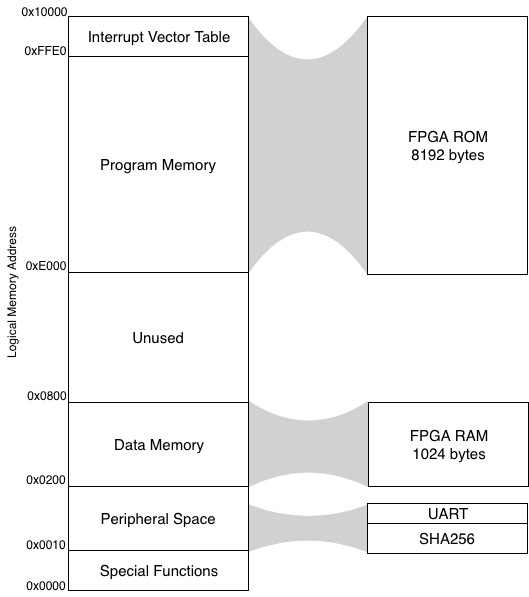
\includegraphics[width=0.6\textwidth]{figuras/original_bus}
	\caption{Memory map using a ROM with 8192 bytes and RAM with 1024 bytes. Also, there are two peripheral, one responsible for controlling the serial communication (UART, universal asynchronous receiver/transmitter) and other to calculate SHA256 hashes.}
	\label{fig:original_bus}
\end{figure}

The scheme showed in the picture are almost the basic MSP430 memory map. The unique difference is the addition of two peripherals to made particular tasks. Using the peripheral directed attached to the memory make easy write and read values from it. Peripherals can be physically added to the microcontroller or can be built into the same integrated circuit. 

When we talk about memory, we have two types of addresses: logical and the physical address. The logical is used by the program to refer to the memory area that it wants to access. The physical one is the address of the device memory. The distinct of this two types is important because in this theses sometimes will be a reference to one type or other.

Make a clear difference between this types, let's give an example. Suppose a program wants to write an integer value (2-bytes) in the address physical address $0x0200$. When the processor runs this instruction, it will calculate the physical address and output this value in the data memory address bus to communicate with the memory. In this example, the value of the physical address will be $0\mbox{x}000$ ($\mbox{\small{LOGICAL\_ADDRESS}}= 2 \times \mbox{\small{PHYSICAL\_ADDRESS}} + 0\mbox{x}200$). The number $0\mbox{x}200$. The number $0\mbox{x}200$ are a default value used by the MSP430 family.

How the MSP430 and its functions works are well known, but how these things are implemented on a hardware level is an industry secret. However, Olivier Girard created an open implementation of the MSP430 in Verilog and made it public under the GNU Lesser General Public License. This project was named openMSP430. This thesis will use the this open version to make changes and implement SMART.

Already has been said that the main difference of models in the MSP430 family is the RAM and ROM memory size. Using the openMSP430 this two value are fully configurable, that is, using the same code is possible to simulate multiple devices. To make things simple, all tests will use a ROM with 8192 bytes and RAM with 1024 bytes, like shown in figure \ref{fig:original_bus}. These two sizes are chosen intrinsically, but they are enough to save and execute programs with a reasonable complexity.

To build the binary code to run in the openMSP430 Texas Instruments use a derived version of GCC\footnote{\url{http://www.ti.com/tool/msp430-gcc-opensource}}. This compiler accepts flags to describe the target device. Also, it supports a memory linker scripts to build the executable to devices that use the MSP430 instruction, but do not correspond to any device of the family. 

This compiler additionally came with the MSP430 header files. Some crucial tasks are the responsibility of these files.  For example, when we declare a string (array of chars), this data will be saved in the ROM memory (the only memory that will be preserved between device resets). If the microcontroller program has an instruction to change one byte of this string, this cannot be done in the ROM. To solve this problem, the compiler inserts a code to be run when the device start. This code has responsible for copying all initialized variables to the RAM. Also, the compiler changes the reference of these variables to point it to the RAM.

There are many other specifications of this microcontroller. The main ones were mentioned here or will have a subsection discussing its.  Other specifications are outside the scope of this work. 

\subsection{Development Board and SPARTAN 6}

A Mimas V2 Spartan 6 FPGA development board is used to test and develop the SMART implementation. This development board has several components to make possible its use in different scenarios. Its manufacture website\footnote{Numato Website: \url{http://www.ti.com/tool/msp430-gcc-opensource}} has a list of all the board components and specification. Here we will discuss some of them.

The SPI flash memory of 16 Mbytes (M25P16) is responsible for saving the Bitgen file, as explained in the diagram. Unfortunately, the programming of this memory is made using a PIC microcontroller that interfaces it with the USB. Because this type of connection and data conversion, there is a significant delay in writing the Bitgen to this memory. 

This PIC microcontroller also serves as a USB-UART interface, which helps to establish the communication between the code in the FPGA and any application running on the PC. Data can be sent and received from the FPGA by using a serial terminal at the fixed of baud rate 19200. This interface will be connected to the UART openMSP430 peripheral, making possible to exchange information between the computer and the microcontroller.

Because the PIC can have two different functions, there is a switch to select the required function.

Some LEDs, buttons, and switches are present in the development board. The switches are used in the hardware tests to help to turn on/off some modules and peripherals. The LEDs are used to show the internal status of the microcontroller. Moreover, one button is used to be the openMSP430 reset pin.

Despite all the components, the principal one is the Xilinx Spartan 6 XC6SLX9 in a CSG324 package with a speed grade of 2. This component as pins connected to all the other devices. Inside it, also has some pre-built components (these components need to be connected using a specific HDL code), like a RAM memory. This model of FGA has 576 Kbytes of RAM. This memory will be used in the implementation to supply the ROM, and RAM needs by the openMSP430. Note that we will use a RAM as a ROM, this not implies in any security fault, because the memory openMSP430 memory backbone prevents any the ROM to be writable.

A considerable time amount of this thesis is spent adapting the openMSP430 implementation to run in the Spartan 6 and this development board. Several times all computer simulating tests in the run without any errors, but when tried in using a real FPGA the tests stopped to work. Unfortunately, to discovery and debug these problems are a difficult task because it involves real hardware. It was necessary to use an oscilloscope several times.

\subsection{Time Constants}

One important thing when working with FPGA is the time constants. These values are essential for testing, and the dispose of the connections inside the FPGA.

For Verilog simulations, the time constants are set using a reserved macro named \verb|timescale|. This macro receives two values: the time unit and time precision. The simulations delays and any time value use the time unit. And the time precision is used by the simulator to know how they can round the summation values. In the tests are used $1ns$ for time unit and $100ps$ for precision. 

\begin{lstlisting}[caption={Simulation clock signal generator.},label={code:clock}]
initial
	begin
		CLK_100MHz = 1'b0;
		forever #5 CLK_100MHz <= ~CLK_100MHz; // 100 MHz
	end
\end{lstlisting}

Code \ref{code:clock} is used in simulation to generate the clock signal. It changes the value of wire \verb|CLK_100MHz| in intervals of $5ns$ (5 units of time), making an output signal of $100MHz$. Is chosen the frequency of $100MHz$  because the testing FPGA has a clock of this frequency. These values are calculated using the frequency formula $F = \frac{1}{T}$, where $F = 100MHz$ is the desired frequency and $T$ is the period. After solving this equation $T = 10^{-8}s$, this is equal to 10 units of time (10ns). The FPGA clock uses a duty cycle of $50\%$, that is that the clock will need to be $50\%$ of their time active and the other part inactive (the signal will change to high to low or vice-versa in an interval of 5 units of time). 

The communication with the simulator in testing or the computer in a real FPGA is made using the RS-232 standard. This standard is a serial protocol, the bits are sent one by time. A direct consequence is that the protocol use time constraints to send the information. In all test is used the 19200 bit$/s$ baud rate, making each bit transmission time be $52100 ns$.

To reduce the timing conflicts and problems inside the openMP430 [\citenum{open}] the microcontroller will receive a clock input of $20000MHz$. To change from $100000MHz$ to the desired input speed, a Digital Clock Manager (DCM) \cite{dcm} will be used.  The DCM is a dedicated hardware inside the FPGA for clock frequency conversion. To this module works it needs several configuration parameters, to simplify it a module named \verb|clock.v| was created with all configurations inside it.

The microcontroller uses one hardware peripheral to interface with the RS-232  serial port. This hardware need to know the bit transmission time, in all software that uses serial has the \verb|UART_BAUD = BAUD;| line. This line is responsible for setting a unique memory address to the correct bit transmission time.

%% 10^9/x*2 = 100*10^6

\subsection{SHA256}
\label{sha256}

One improvement in this implementation compared to the original article has using a hardware SHA2 (Secure Hash Algorithm 2) to hash the memory. The original implementation uses a software SHA1. Different from SHA1, SHA2 is a family of hash function, in implementation use the SHA256 function. 

The SHA256 has some improvements compared to the SHA1. The first one has the input size,  SHA1 needs to receive only 160 bits to produce a hash, the SHA256 needs 256 bits. SHA1 was deprecated by NIST (National Institute of Standards and Technology) in 2011. There also some articles, like \cite{dangersha1},  to show how an attacker can forge two distinct PDF documents with the same SHA-1 hash.

It is important to notice that exist a new version of the secure hash algorithm, the SHA3.  This version made some improvements and NIST advise to use it. There was the attempt to implement the SHA3 in the FPGA, but it exceeds the number of available LUTs in the FPGA, making the implementation impossible with the openMSP430 core. However, SHA256 is still considered segure, and it fit inside the FPGA. 

A SHA256 implementation written by Joachim Strombergson \cite{hash} has used. A peripheral adaptor was built to communicate with the openMSP430 core. This adaptor is responsible for interfacing the SHA3 implementation with the peripherals pins in the microcontroller. The file \verb|SMART/rtl/verilog/sha256/sha256per.v| contains this interface.

Another change is the use of a hardware hash function and not a software one.  This change makes the hash timing faster and saves several bytes in ROM. However, it uses  approximately 2000 FPGA LUTs.

\subsection{SMART Memory Access Control}
\label{smart_mac}

A specific module was developed to build one hardware that guarantees the A3, A5, and A6 assertions. We give the name of SMART Memory Access Control (SMART MAC) to this module. It usually needs to be between the microcontroller and the memory that we want to protect.

To of full comprehension of this module and its capabilities, table \ref{table:smart_mac_pins} show all hardware pins it has and the table \ref{table:smart_mac_parans} shows all parameters.

\begin{table}
	\begin{center}
		\begin{tabular}{|l|c|c|@{}m{8.5cm}@{}|}
			\hline 
			\textbf{Port Name} & \textbf{Direction}& \textbf{Width}& \textbf{Description} \\
			\hline 
			\verb|in_safe_area| & Output& 1 bit& This pin becomes HIGH between the moment the \verb|ins_addr| point to the \verb|HIGH\_SAFE| address to the moment it exits from the safe code area.  \\
			\hline 
			\verb|reset| & Output& 1 bit& This pin becomes HIGH when some violation occurs and a microcontroller a reset is needed. \\
			\hline 
			\verb|mem_dout| & Output& 16 bits& If no violation occurs and all states are correct this value will be equal \verb|mem_din|. Otherwise will be 0x000. \\
			
			\hline 
			\verb|mem_addr| & Input& variable & Memory physical address. \\
			\hline 
			\verb|mclk| & Input& 1 bit& Microcontroller clock. \\
			\hline 
			\verb|mem_din| & Input& 16 bits& Memory data input. \\
			\hline 
			\verb|ins_addr| & Input& 16 bits& Instruction pointer logical address. \\
			\hline 
			\verb|disable_debug| & Input& 1 bit& When this pi is HIGH, the module will be disabled. This feature is used for debug propose. \\ 
			\hline
		\end{tabular}
	\end{center}
	\caption{This table describe all the input and output pins in the SMART Memory Access Control (SMART MAC). When using this module with a real FPGA, only the pin in\_safe\_area can be not connected to the circuit. To make the module work uninterrupted the pin disable\_debug can be continuously set to zero.}
	\label{table:smart_mac_pins}
\end{table}

\begin{table}
	\begin{center}
		\begin{tabular}{|p{4cm}|p{10cm}|}
			\hline 
			\textbf{Parameter Name} & \textbf{Description} \\
			\hline 
			SIZE\_MEM\_ADDR & width of \verb|mem_addr| \\ 
			\hline 
			LOW\_SAFE &  The lower physical address in the region's memory to be protected.\\ 
			\hline 
			HIGH\_SAFE & The higher physical address in the region's memory to be protected. \\ 
			\hline 
			LOW\_CODE & Where the function that will access the protected region in memory begins. Virtual address. \\ 
			\hline 
			HIGH\_CODE & Where the function that will access the protected region in memory ends. Virtual address. \\ 
			\hline 
		\end{tabular}
	\end{center}
	\caption{When building a module using Verilog is possible to insert some parameters. This table is the list of all possible parameters and it description of the SMART Memory Access Control (SMART MAC) module.}
	\label{table:smart_mac_parans}
\end{table}

This basic module idea is to monitor the current instruction pointer address and depending on its position allows the access to a specific memory region. We will call this area as the protected memory region. If there is any trial to access this region when the instruction pointer is in an invalid position the module will send a reset signal to the microcontroller.

Most specifically, the protected memory region will only be readable when an internal module register is activated.  This activation happens when the instruction pointer points to the first instruction of a specific function (the LOW\_CODE and the HIGH\_CODE parameters describe the place of this function). After it is activated, the deactivation only occur if the instruction pointer is outside the function addresses area. The protected memory region is described by the LOW\_SAFE and the HIGH\_SAFE parameters.

A single SMART MAC can be used in the memory bus to make the A3 assertion valid. In this case, the memory protected area will be the key and the allowed function to read it will be the smart function.

To assertion A5 be valid a SMART MAC is used differently. Suppose the smart function started it code in $X$ and ends in the $Y$ logical memory address. A module will be built with: LOW\_SAFE = $X'+2$ byte,  HIGH\_SAFE = $Y'$, LOW\_CODE = $X$  and HIGH\_CODE = $X$.  $X'$ and $Y'$ are the physical memory address derived from the logical addresses. We add two bytes to the physical memory address of the SMART function because it is outside the protected memory region (the first instruction is not protect).

Also, assertion A6 is guaranteed by module this second module, because if the instruction pointer goes outside the function memory region, the function can only be callable from it beginning. If someone tries to call this function by its middle, a reset signal will be produced.


% speak of one

% puting docgether

\begin{figure}[h]
	\centering
	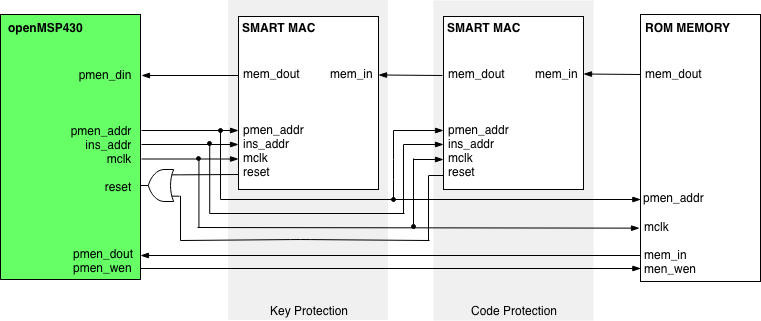
\includegraphics[width=0.9\textwidth]{figuras/smart_mac}
	\caption{The interface between the ROM memory and the openMSP430. In the middle, is SMART memory access control module. }
	\label{fig:smart_mac}
\end{figure}

Using two SMART MAC is possible to grant the three remaining assertions. In figure \ref{fig:smart_mac} is possible to how these modules are placed between the microcontroller and the memory. Note that the left module is responsible for protecting the key and the right one to protect the code.

The original SMART article changes the openMSP430 memory backbone to validate the A3, A5, and A6 assertions.  With the creation of SMART MAC, there was a much less invasive modification the microcontroller and produce the same guarantees. Besides that, the use of a module that does not make changes in the core elements of microcontroller make the solution more portable to other platforms. 

Appendix \ref{cap:apendiceA} make a deeper analysis of SMART MAC. Also, it contains the module core code\footnote{The SMART MAC source file is in the \mbox{\textit{SMART/rtl/verilog/smart\_mac.v}} directory of this thesis repository. The implementation of the connections described in figure \ref{fig:smart_mac} is present in the \mbox{\textit{SMART/rtl/verilog/openMSP430\_fpga.v}} directory. }.

\subsection{Linker Script}

When building the binary source to a microcontroller the compiler needs to know where to place the code, data and other pieces of information in the memory. Linker script (or linker command file) is a particular file that describes to the compiler this attributes.


\begin{figure}[h]
	\centering
	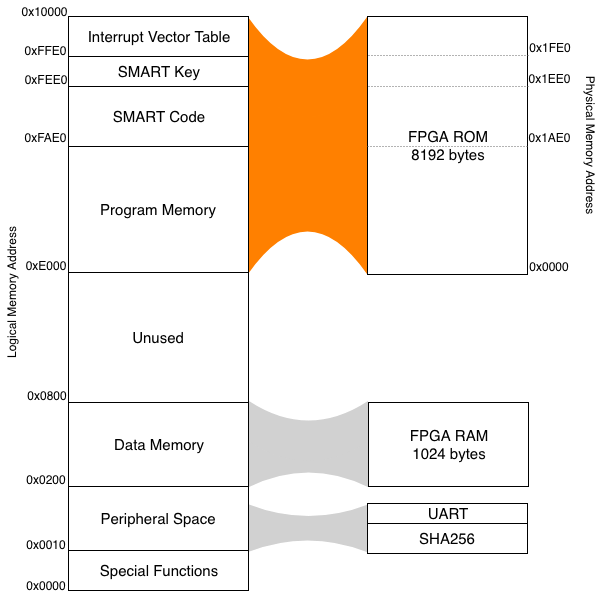
\includegraphics[width=0.6\textwidth]{figuras/smart_bus}
	\caption{The orange link is the program memory backbone where the smart modules are introduced. Differently, from figure X, this image includes de physical and logical addresses used by the SMART code and the SMART key. }
	\label{fig:smart_bus}
\end{figure}

In figure X is possible to see where the SMART MAC was implemented. Also, this image contains information about the new memory sections created for salving the SMART key and code. It was not quoted before, but the image has a special section named \textit{Interrupt Vector Table}. This memory region has 16 processor addresses (the equivalent of 32 bytes) and in there is functions addresses to be callable when one interruption occurs.  The first 16-bit word in this section (address 0xFFFE) is the instruction that the processor will jump and a reset is performed.   There is an importance to do not block this memory sections because it provides primordial functionalities to the microcontroller. 

Shortly after this section of memory was introduce a memory protect region to save the SMART key. The linker script described this section, that way the compiler will not introduce any code in there. A particular attribute was used in the C source code to force the key to be kept in that region. The SMART key memory region starts at byte 0xFEE0 and has a length of  0x0100 bytes.

A region for SMART code is also introduced. It starts at byte 0xFAE0 and has a length of 0x0400 bytes. All the smart code will be saved in this is the memory section. Because of that, this section can contain multiple functions. Depending on the order the header of this functions are declared the compiler can locate one function after other. As a consequence, the main SMART code function needs to be the first declared. Otherwise, if the SMART main function is not at the first address, its call will not unlock it executable source and will provoke an unexpected reset. That is, in the SMART code, the order of the function header matters.

The linker script can be found in \verb|SMART/software/libs/linker.msp430-elf.x| file. This script was based the original linked script provided by Texas Instruments.

\section{Tests}

This section explains how SMART implementation was tested. The last subsection will show a real application using SMART. 

\subsection{Continuous integration}

A continuous integration system is used to prevent and identify any code error or change that affected the correct work of the microcontroller. A GitHub project is set to track the code changes and versioning the code.  On every push, a server receives a notification, run all test in the project and build the FPGA files. 

Jenkins\footnote{https://jenkins.io/} is used to build the continues integration system. Other systems, like Travis or Gitlab CI, are not used because they have restrictions on the maximum size of their builds. To test and mount the code the ISE WebPACK Design Software is used, which has  6 GBytes. Jenkins makes possible install this software on the tester machine only one time and uses it when needed. 

Two simulation softwares are used to reproduce the behaviour of the hardware: the Icarus Verilog\footnote{http://iverilog.icarus.com/} (an open-source project) and the Xilinx ISE (a property software). Every test is executed using this two simulation softwares. This decision was made because during the development are notice that some errors only occur in one of them and not in the other or vice-versa.

\subsection{Light Remote Control}

To test and study SMART, a full application is built using it. The basic idea was to build a device able to receive remote commands to turn off and on this led with all the security guarantees. As said before, this device was built in an FPGA, that run the openMSP430 project with two SMART MAC modules in the memory bus.  As the most IoT devices, it runs as client on the internet. Because of that, a simple python server was written to answer the requests, save the device key and to calculate the expected hash values.

\begin{figure}[h]
	\centering
	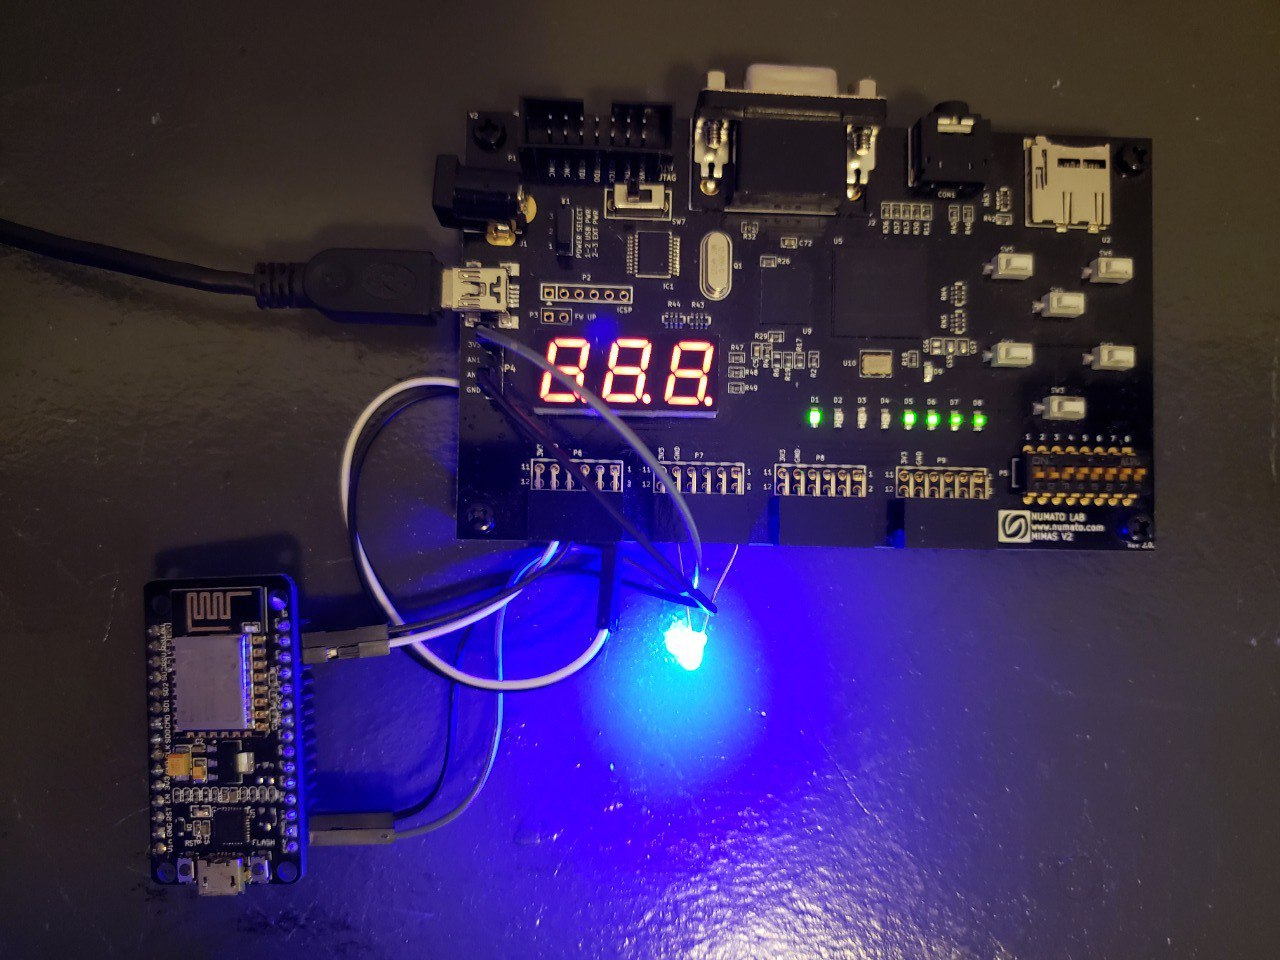
\includegraphics[width=0.50\textwidth]{figuras/real}
	\caption{The Numato Mimas V2 (in the right) connected with an Amica Node MCU (in the left) board with the ESP8266 module. A wall charger supplies the device by the USB port.}
	\label{fig:real}
\end{figure}

In figure X is possible to see the final hardware in this application. An ESP8266 module was used to make the FPGA able to connect to the internet. A small software was written to this module control the connection to the internet and  among this two devices. It creates a TCP connection between it and the server. All data received by internet is streamed to the FPGA serial connection and, if the FPGA send any byte, the module gets the byte and sent to the TCP connection. The ESP866 module was programmed using the Arduino environment with the Arduino core for ESP8266 WiFi chip\footnote{url{https://github.com/esp8266/Arduino}}. 

IN the implementation this module was not attested. That is, if it suffers any attack it will not be detected. However, it is possible to connect some pins of this module to allow the FPGA to read it internal memory. Making it is possible to create an attestation algorithm to validate this module memory. Note that, this algorithm will be a program in the openMSP430, this program can be attested using the SMART functions.

Because the connection between the two devices is made using the serial protocol, some problems have arisen. There is no attempt to change to other protocol because this protocol is simple to use and we already had an HDL implmentation of a peripheral with this protocol.  The main problem is that some bytes are getting wrongly when the internet module send it the FPGA. To counter this problem, a particular communication protocol was written. 

On the other side of the communication channel, there is a Python server responding all the requests. The \textit{socketserver} library was used to implement the server. This library help t create a new process to handle a connection, this enables multiple connections at the same time. Unfortunately, the server was hardcoded the device key and the path to its source code. In a real application, each device must have a unique key and a database stores all this data. 

The device was responsible for creating the TCP connection, but when performed, only the server can send commands to it, and the device only becomes responsible for responding to the requests. This protocol has only five commands: 

\begin{itemize}
	\item \verb|TAKE_HASH|: used to server request a hash from a memory area. The smart code is responsible for calculating this hash. A 256 bits hash is expected as a response to this command.
	\item \verb|SET_LED_ON|: turn on the led. 
	\item \verb|SET_LED_OFF|: turn off the led. 
	\item \verb|SET_RESET|: forces a reset in the device. 
	\item \verb|GET_RESET_HASH|: if a reset is successfully made, it will produce a hash from the previous command. This command is responsible for requesting this hash from the device. 
\end{itemize}

As said, a protocol is designed to send this commands. On every server request, 263 bytes are sent to the device. The first byte is the command byte. Each command has a byte associated with it. The device will receive it and call the correct functions after that. The next two bytes (16 bits) are a memory address number that will be used to start the hash computation. Next, there are more two bytes, that represent how many bytes will be part of the hash. The next 258 bytes are part of the attest nonce. These bytes can be divided in three section of 86 bytes, each section is equal with each other. This decision was made because if any byte gets wrongly by the device, it can restore the original one. 

To compute the hash, the device uses a nonce of  256 bytes.  Because the serial connection error, an error-correcting algorithm was used.  Algorithms like the Hamming code can be able to correct errors with a small overhead in the connection. However, these algorithms are complicated to implement and uses a lot of the memory of the microcontroller (only 5120 bytes are available is the program memory). As a solution, the nonce size has reduced and sent three times. The reduction is necessary the save the data memory. Using this method, became easy to correct any communication error. 

Also, to reduce the communication error a low baud rate of 4800 bit/s was used. Another method to reduce this errors would be soldering the internet module in the FPGA, but this would damage the test devices.

For all server commands, the device needs to send a response. However, for only the commands \verb|TAKE_HASH| and \verb|GET_RESET_HASH| this response need to be a valid 256-bit hash. With this hash, the server became able to attest the device remotely.  In the device response to the server are not any error prevention measures.

To test the protocol and the SMART functionality a simple communication mock has built. First of all, the server asks for a hash from the address 0x0000 with 0 bytes. Although this command does not appear useful, it cam detected if the correct device is connected with the server. Id other device connected, it will not be able to produce the expected hash. After that a \verb|SET_LED_ON| command is sent. Nest, the server asks for a hash from the led status variable address with 1 byte to verify if this command takes effect. Again, if the value was not the expected one, the hash will be incorrect. In the mock, this verification is made ten times with a small time interval between them. The same procedure is repeated turning off the led.

After that,  is requested a hash of the full program memory. The response of this request is important to see if the device code has not changed. To verify if this function is correctly working some untrusted code was injected into the device and was successfully identified. To make is identification more precisely, the server several requests different memory blocks, following a binary search algorithm. As a result, we obtain the first changed byte. 


Subsequent the code verification,  a reset signal is sent. The hash computes from the information send by this command is preserve in the hash peripheral, becoming available after the reset. After 5 seconds, the server sends the \verb|GET_RESET_HASH| command to retrieve this hash and verify if a successful reset was made.

In the server and the device are set timeouts if some errors occur. These timeouts are essential because if any the internet connection or the cable between the devices fail, the server and the device will know how to handle this problem. 

Two attacks are made to test this implementation. The first one is a man-in-the-middle attack. In this attack every time the command \verb|SET_LED_ON| was sent, the attacker changes the command to \verb|SET_LED_OFF| and vice-versa. As a result, all the verification of led variable value produces an unexpected hash value, proving that the device or the connections have been changed. The attack is made making an ARP spoofing, changing the packets change in a specific port and redirecting the data.

Note that during this procedure, the attacker successfully changes the led status. This problem happens because the device cannot identify the server. One way to mitigate this attack is the device generate a random number and make a hash of it. After that, the device must send this random value and ask for the server the expected hash value. If the server returns the correct value, the device can confirm that is the correct server. Unfortunately, the openMSP430 did not come with a random number generator to make this feature viable. Generate a random number in this microcontroller unit an be part of future work.

The second attack was made by changing the code of the device. When this happens, the function responsible for calculating the hash from the program memory return an incorrect value. 

Other information about this test and the source code are in the main code repository.

% acender luz
% vou mandar o valor via rede, 0 ou 1 e a luz vai ascender ou apagar. A cada comando é retornado o hash do dispositivo. Vamos ter um beffer seguido de uma contante que salva o valor atual da luz. Esse bufer vai ter uma posiçao, vai ser possivel fazer um overflow dessa posicao e mudar o estado da luz.

% meu servidor manda aordem de estar apagado, verifico o estado e esta tudo ok
% meu servidor manda a ordem de apagar, um fdp vai e muda, meu servidor pergunta o status e pinba, pega que ta diferente do esperado. -> ataque na rede

% podemos salvar o substantivo no dispositivo e ter. Vamos verificar se o ultimo enviado foi o veridico e o esperado.

% no exemplo acima é possivel verificar se o cara que enviou é o detentor da minha chave. Ele envia o sha do substantivo e se eu criptografar e bater, tomo a atitude.

%-------------------
% estouro a pilha e causo um reset....
% ver

\section{Results}

\begin{table}
	\begin{center}
		\begin{tabular}{|p{4cm}|c|c|}
			\hline 
			& \textbf{Number of Slice Registers} & \textbf{Number of Slice LUTs} \\
			\hline 
			SMART without SHA256 peripheral & 1025 & 2492 \\
			\hline 
			SMART with SHA256 peripheral & 2702 & 4764 \\
			\hline 
			MCU with SHA256 and without SMART & 2694 & 4710 \\
			\hline 
		\end{tabular}
	\end{center}
	\caption{Use of the FPGA LUTs and registers depending activation of SMART and the SHA256 peripheral.}
	\label{table:results}
\end{table}

As a result of the tests are obtained table \ref{table:results}. This table shows that the SMART implementation in the memory bus uses a small number of LUTs and registers. However, using a hardware implementation of the hash function almost double the necessary hardware. Unfortunately this is not a good thing, because one of the main objectives is to maintain a lower device cost.

One way to solve this problem is to expand the device program memory size and use a software SHA256 hash implementation.  This changes also increase the cost of the device. By the Xilinx Spartan 6 manual, each slice can store 8 bits of information, that is, one byte. The SHA256 software uses approximate 1300 bytes of memory \footnote{This value is obtained running the tool msp430-elf-size in the with and without a software SHA256 implementation. The source for the hash code was obtained in the RFC4634.}. That is, the cost of using a hardware version will be a little more significant, not 180\% as shown in table \ref{table:results}.

Another significant result obtained was the hash computation time in the network, that is the device response time after a command to compute a hash. The theoretical computation time from the hash peripheral can be obtained from the hash source code. This value is not so interesting, because it is count in the number of the clock cycles and does not involve any variation.  0.72 seconds was the average time response after a \verb|TAKE_HASH| command in the Light Remote Control experiment. This result was obtained after 1000 measures, using one byte to compute the hash. The experiment was run in a local network, with the computer as a server and the device, both connected by wireless with a 2,4 GHz Wi-Fi  (manufacturer Askey  and model RTF3505VW-N1).

Another similar test was run. But, instead of asking the hash of one byte, was requested the hash of  8192 bytes. 0.73 seconds is the average obtained.  This little change in this scenarios shows that most of the time is used by the communication and the pre-processing computation and not for the hash calculus. Probably this time has significant because of the serial protocol between the FPGA and the wireless module.

